\documentclass[english,a4paper,12pt]{article}
\usepackage[T1]{fontenc} %for å bruke æøå
\usepackage[utf8]{inputenc}
\usepackage{graphicx} %for å inkludere grafikk
\usepackage{verbatim} %for å inkludere filer med tegn LaTeX ikke liker
\usepackage{amsfonts}
%\usepackage[framed]{mcode} %for å få inn matlabkode
\usepackage{listings}
\usepackage[margin=1.2cm]{caption} % skalere figur text
\usepackage{subfigure}


%\bibliographystyle{plain}
\usepackage{parskip}
\usepackage{babel, textcomp, color, amsmath, amssymb, tikz, subfig, float}
\renewcommand{\captionfont}{\sffamily\small}
\renewcommand{\captionlabelfont}{\bf}
\fboxsep=0mm % ramme inn bilder

\title{FYS3150 - Exam Project}

\author{Kandidate 3}

\date{\today}

\begin{document}
\maketitle

\begin{center}
 DIFFUSION IN TWO DIMENSIONS
\end{center}


\begin{center}
GIT hub link: https://github.com/steffemb/project5/tree/master/
\end{center}

\newpage

\section*{Abstract}


\section*{Introduction}

In this project i will discuss project 4 briefly. We are going to implement the Explicit, Implicit and Crank Nicholson
schemes for solving 1+1 dimensional partial differential equations (PDE).

We will discuss strength and weaknesses of using Markov Chains to solve PDEs in 1+1 and 2+1 dimensions. We wish to
get insight in to strengths and weaknesses of the different methods, and compare them.

There are many situations where we wish to solve PDEs similar to the diffusion equation. We use many similar equations in 
everything from meteorology to simulations of quantum systems, and it is therefore not hard to imagine that there area different
situations where different methods are the easiest, or most effective to implement. 


\section*{Solution}

\subsection*{1+1 Dimensional Diffusion equation, explicit and implicit solvers}

I will firs recap project 4. In project 4 we solved th diffusion equation with an explicit, implicit, and a Crank Nicholson scheme.

the equation we solve in 1+1 dimensions is:

\begin{equation}
D \frac{\partial^2 u(x,t)}{\partial x^2} = \frac{\partial u(x,t)}{\partial t}
\end{equation}

with initial conditions $u(x,0) = 0, 0<x<d$, and $u(0,t) = 1, t>0$, and $u(d,t) = 0, t>0$, For the rest of the project we can set $D=1$.

First we write a code for the explicit Euler scheme. Mathematically this is written:

\begin{equation}
\frac{u(x_i,t_j+\Delta t)-u(x_i,t_j)}{\Delta t} = \frac{u(x_i+\Delta x,t_j)-2u(x_i,t_j)+u(x_i-\Delta x,t_j)}{\Delta x^2}.
\end{equation}

This is fairly easy to write an algorithm for, we only need to solve for $t_j + \Delta t$, and we get the equation:

\begin{equation}
u(x_i,t_j+\Delta t) = u(x_i,t_j) + \frac{\Delta t}{\Delta x^2} u(x_i+\Delta x,t_j)-2u(x_i,t_j)+u(x_i-\Delta x,t_j).
\end{equation}

The algorithm now only needs a for loop over j, and i, which is the time and space indexes. Note that the i indexes must exclude
the first and last indexes.
The second task is to implement the Implicit Euler scheme. We start with the mathematical expression:

\begin{equation}
\frac{u(x_i,t_j)-u(x_i,t_j-\Delta t)}{\Delta t} = \frac{u(x_i+\Delta x,t_j)-2u(x_i,t_j)+u(x_i-\Delta x,t_j)}{\Delta x^2}.
\end{equation}

This time we solve for $t_j - \Delta t$, and we get:

\begin{equation}
u(x_i,t_j-\Delta t) = u(x_i,t_j) - \frac{\Delta t}{\Delta x^2} u(x_i+\Delta x,t_j)-2u(x_i,t_j)+u(x_i-\Delta x,t_j)
\end{equation}

Lets define $\alpha = \frac{\Delta t}{\Delta x^2}$. And rewrite the equation as a linear equation.

\begin{equation}
u(x_i,t_j-\Delta t) = u(x_i,t_j) -\alpha \hat A u(x_i,t_j),
\end{equation}

where $\hat A$ is the matrix:

\begin{equation}
{\bf A} = \left(\begin{array}{cccccc}
-2& 1& 0 &\dots & \dots &0 \\
1 & -2 & 1 &0 &\dots &\dots \\
0&1 &-2 & 1 & 0 & \dots \\
& \dots & \dots &\dots &\dots & \dots \\
0&\dots & &1 &-2& 1 \\
0&\dots & & 0 &1 & -2 \\
\end{array} \right)
\end{equation}

further:

\begin{equation}
u(x_i,t_j-\Delta t) = u(x_i,t_j)(\hat I -\alpha \hat A),
\end{equation}

And we can define:

\begin{equation}
\hat B = (\hat I -\alpha \hat A)
\end{equation}

\begin{equation}
{\bf B} = \left(\begin{array}{cccccc}
1+2\alpha& -\alpha& 0 &\dots & \dots &0 \\
-\alpha & 1+2\alpha & -\alpha &0 &\dots &\dots \\
0&-\alpha &1+2\alpha & -\alpha & 0 & \dots \\
& \dots & \dots &\dots &\dots & \dots \\
0&\dots & &-\alpha &1+2\alpha& -\alpha \\
0&\dots & & 0 &-\alpha & 1+2\alpha \\
\end{array} \right)
\end{equation}

Now scince $\hat B = \hat B^{-1}$, $ u(x_i,t_j) = \hat B u(x_i,t_j-\Delta t)$. This we can solve with a forward and backward substitution.
-----------------For details see project 1.-----------------------

The last task is to implement the Crank Nichols scheme. We can here also start with the mathematical expression:

\begin{equation}
\begin{split}
\frac{u(x_i,t_j+\Delta t)-u(x_i,t_j)}{\Delta t} = \frac{1}{2}\left(\frac{u(x_i+\Delta x,t_j)-2u(x_i,t_j)+u(x_i-\Delta x,t_j)}{\Delta x^2}+\right. \\
\left. \frac{u(x_i+\Delta x,t_j+\Delta t)-2u(x_i,t_j+\Delta t)+u(x_i-\Delta x,t_j+\Delta t)}{\Delta x^2} \right).
\end{split}
\end{equation}

This expression can be a bit misleading. If we stare a bit at this equation we see that there are two parts that look the same as
in the two schemes above. What isn't clear in eq. 10 is that we wish to solve with the explicit scheme first and the use tis solution
in the implicit. It really is as easy as that but let me clarify a couple of details first. We rewrite the equation:

\begin{equation}
\begin{split}
2(u(x_i,t_j+\Delta t)-u(x_i,t_j)) = \alpha\left( (u(x_i+\Delta x,t_j)-2u(x_i,t_j)+u(x_i-\Delta x,t_j)) +\right. \\
\left. (u(x_i+\Delta x,t_j+\Delta t)-2u(x_i,t_j+\Delta t)+u(x_i-\Delta x,t_j+\Delta t)) \right).
\end{split}
\end{equation}

We see that we get a factor of two which changes our $\hat B$ matrix, so $ \hat B' = (2 \hat I -\alpha \hat A)$
and the algoritm is now simply:

1. solve u(x,t) with explicit scheme.

2. put these u(x,t) values into the implicit sceme and solve using the $\hat B'$ matrix.

3. put u(0,t) += alpha

The last point is a cool trick to let us solve for u staigt away without changing to ``simpler'' boundary conditions.
This comes from the first row of matrix $\hat B'$. In project 1 we had a matrix with two fictive points in the begining and end
that where 0. So they gave us no problems. Now the points are $-\alpha$. if we write out the equation it gieldes, it goes as follows:

\begin{equation}
-\alpha u_0 + (2+2\alpha) u_1 - \alpha u_2 = u_1 \Rightarrow (2+2\alpha) u_1 - \alpha u_2 = u_1 + \alpha
\end{equation}

So we simply add $\alpha$ to the first entry.

\subsection*{1+1 Dimensional Diffusion equation, Markov Chains}

We will now build up a system for solving the diffusion equation as a Monte Carlo experiment. To do this we will use Markov Chains.
Markov Chains are often ``intuitively'' pleasing in the sense that the algorithm is built up based on ``intuition'' of the real world.
In our simulation based on Markov chains we will not need any mathematical deduction, we will merely set up a box and push particles in
to this box and then let each particle float randomly around. What makes Markov chains neat, and in many cases simple and intuitively pleasing,
is that the next state of the system only depends on the current state of the system, and not the sequence that precedes it.

We first need to set up a system, some way to store the information about each particle. To make the code readable i made a class ``system''
that contains a vector of class objects ``particles''. Each particle in ``particles'' has properties x, and y position. Although we will only
use x-position in 1+1 dimensions. The class ``system'' also has a function ``add particle'' which adds a new object ``particle'' to the vector at x-position = 0.

We then call ``add particle'' $N=10^4$ times to set up the initial state of the system.

We need to set up rules for the particles:

1. For each time step we iterate over each particle, for each particle we draw a random number in the interval [0,1].
If the random number is <= 0.5, move the particle a distance $-l_0$, or if the random number is > 0.5, move the particle a distance $+l_0$.

2. No particle can exist outside the box. In 1+1 dimensions we have a ``dimensionless'' box with unit length 1. If a particle moves outside the box, 
delete it.
this is equivalent with having boundary conditions equal to zero when solving the diffusion equation.

3. we want a steady stream of particles from one side. We therefore set up an area from 0 to $l_0$ where there is only allowed to be
$N=10^4$ particles. And not less. This can be solved in different ways, but i found that the most dynamic way was to have a counter with
the number of particles in this area. If a particle is in this area and moves out, we do a ``counter -=1''. And if the particle is outside this
area and moves in to it we do a ``counter += 1''.
When implementing this rule for the particles it is equivalent with having a boundary condition at zero equal to one.
I will explain later why it is equal to one and not $N$ when we build a histogram.

Next we need to build a histogram over density of particles. We wish to build a histogram for each time step so that we can plot the development
in time of the system. I decided to set up a histogram of step length $l_0$. So the histogram is dynamic and follows the step length of the particles.
to fill the histogram we need a function that iterates over all particles and counts up how many particles are in each step length. We then divide each count of particles
by $N$. This should give a histogram that is one in the first interval and zero in the last so it is easy to compare to the closed form
solution.

Lastly we wish to do all this with a fixed step length and a gaussian step length. The fixed step length is fairly simple to implement.
there should be no problems as long as the histogram is spaced according to the step length, and the step length is then
$l_0 = \sqrt{2D\Delta{t}}$. For the gaussian step we want the mean value of all the step lengths to be $l_0$. we can therefore set
$l_gauss = l_0\zeta$, where $\zeta$ is a random number picked in the normal distribution centered at $0$ with standard deviation $\sigma = \frac{1}{\sqrt{2}}$

\subsection*{1+1 Dimensional Diffusion equation, closed form solution}

We will need a closed form solution of equation (1) to compare to the various numerical solutions. To find this solution we need 
to rearrange the boundary conditions. To find a solution we need boundary $u(0,t) = u(L,t) = 0, t \geq 0$. 
Our final solution will then be $v(x,t) = u(x,t) + u_{s}(x,t)$ where $u_{s}(x,t) = 1-x$ is the steady state solution.

We first assume separation of variables, so: $u(x,t) = F(x)G(t)$. We then get

\begin{equation}
 \frac{\partial^2}{\partial x^2} F(x)G(t) = \frac{\partial}{\partial t} F(x)G(t)
\end{equation}

We rewrite the equation with simpler notation.

\begin{equation}
 \frac{F''}{F} = \frac{G'}{G} = -\lambda^2
\end{equation}

Since we have separated the variables the two sides of the equation must be equal to the same constant. We call it $-\lambda^2$ 
just because we know where we want to go in the end.

This has the general solution

\begin{equation}
 F(x) = A sin(\lambda x) + B cos(\lambda x),\space and \space G(t) = Ce^{-\lambda^2 t}.
\end{equation}

Boundary conditions at $u(0,t) = 0$ gives $B = 0$, and Boundary conditions at $u(L,t) = 0$ gives $F(x=L) = A sin(\lambda L) = 0$
$A \neq 0$ so $sin(\lambda L) = 0$ which gives $\lambda = \frac{n \pi}{L}$, $n = 1, 2, 3...$. Put together the solution has the form

\begin{equation}
 u(x,t) =\sum_{n=1}^{\infty} A_n sin(\frac{n \pi x}{L}) e^{\frac{-n^2 \pi^2 t}{L^2}}.
\end{equation}

$A_n$ is a Furier coefficient, and Furier expansion theory gives

\begin{equation}
 A_n = \frac{-2}{n \pi}
\end{equation}

We let $L = 1$ since that is what we will be simulating and the final solution is

\begin{equation}
u(x,t) = \sum_{n=1} \frac{-2}{n \pi} sin(n \pi x)  e^{-n^2 \pi^2 t}
\end{equation}

\subsection*{2+1 Dimensional Diffusion equation}

We need some sort of closed form solution to test our simulations against. so first we expand the diffusion equation to one more spatial
dimension

\begin{equation}
 \frac{\partial^2 u(x,y,t)}{\partial x^2} + \frac{\partial^2 u(x,y,t)}{\partial y^2} = \frac{\partial u(x,y,t)}{\partial t}.
\end{equation}

This equation is not generally solvable, but we can solve the Laplace equation

\begin{equation}
 \bigtriangledown^2 u_{s}(x,y) = 0,
\end{equation}

which will give us the steady state solution $u_s$. we start again with assuming separation of variables $u_{s}(x,y) = X(x)Y(y)$

we then get 

\begin{equation}
 \frac{\partial^2 u_s}{\partial x^2} = Y \frac{d^2 X}{dx^2},\  \frac{\partial^2 u_s}{\partial y^2} = X \frac{d^2 Y}{dy^2}. 
\end{equation}

these two together with eq (21) gives

\begin{equation}
 \frac{1}{X}\frac{d^2 X}{dx^2} = -\frac{1}{Y}\frac{d^2 Y}{dy^2} = \lambda^2
\end{equation}

so
\begin{align*}
 \frac{d^2 X}{dx^2} = \lambda^2 X,\ \frac{d^2 Y}{dy^2} = -\lambda^2 Y
\end{align*}

These have general solutions on the form

\begin{equation}
 X(x) = \gamma cosh(\lambda x) + \delta sinh(\lambda x),
\end{equation}
\begin{equation}
 Y(y) = \alpha cos(\lambda y) + \beta sin(\lambda y).
\end{equation}

We now insert the boundary conditions:\newline

1. $u_{s}(0,y)= 1 =\gamma cosh(\lambda x) + \delta sinh(\lambda x)$\newline
2. $u_{s}(x,0) = 0 = \alpha cos(\lambda y) + \beta sin(\lambda y)$\newline

from 2. we get either $\gamma = \delta = 0$, or $\alpha = 0$, scince $\alpha \neq 0$ is nontrivial, we chose $\alpha = 0$

and then from 1. $\gamma\beta sin(\lambda y) = 1$, and

3. $u_{s}(x,1) = 0 = \beta sin(\lambda)(\gamma cosh(\lambda x) + \delta sinh(\lambda x))$.

which gives us $\lambda = n\pi, n = 1,2,3....$ 

4. $u_{s}(1,y) = 0 = \beta sin(n\pi y)(\gamma cosh(n\pi) + \delta sinh(n\pi))$

Which gives us $\delta = - \gamma coth(n\pi)$

We now go back to 1.
\begin{align*}
 u_{s}(0,y) = 1 = \sum_{n=1}^\infty \gamma_n sin(n\pi y)
\end{align*}

and from furier expansion we get 

\begin{equation}
 \gamma_n = \frac{2}{n\pi}(1-cos(n\pi)).
\end{equation}

And the final form is then 
\begin{equation}
 \sum_{n=1}^\infty \frac{2}{n\pi}(1-cos(n\pi))sin(n\pi y)(cosh(n\pi x)-coth(n\pi)sinh(n\pi y))
\end{equation}

with this solution we can check if the simulations and solvers are doing what they should after they reach a steady state. We 
will not be able to check if the time development is correct though.

\subsection*{2+1 Dimensional Diffusion equation, PDE solvers}

Lets first look at the explicit scheme. The derivation of this equation is given in the lecture notes chapter 10.2.5

The equation we need to implement is:
\begin{equation}
 u_{i,j}^{l+1} = u_{i,j}^{l} + \alpha (u_{i+1,j}^{l} +u_{i-1,j}^{l}+u_{i,j+1}^{l}+u_{i,j-1}^{l}-4 u_{i,j}^{l})
\end{equation}

Where i, j denotes spatial steps, and l denotes time steps. $\alpha = \frac{\Delta t}{\Delta h^2}$, and $\Delta h = \Delta x = \Delta y$ Here the left hand side is the only unknown term so solving
this is done simply by a double for loop over i, j. The only tricky part is to set up the initial conditions correct, and
set the for loops to go from $1$, to $length-1$ to avoid index errors.

The next task is to implement the implicit scheme with the Jacobi iterative method. Here we also need to implement an equation:

\begin{equation}
 u_{i,j}^{l} = \frac{\alpha}{1+4\alpha}(\alpha(u_{i+1,j}^{l} +u_{i-1,j}^{l}+u_{i,j+1}^{l}+u_{i,j-1}^{l}) + u_{i,j}^{l-1})
\end{equation}

Here we need the solution at the previous time step to find the next. the rest is mostly the same as over.



\subsection*{2+1 Dimensional Diffusion equation,  Markov Chains}

Adding one extra spatial dimension to the Markov chain simulation is fairly easy. Again it is kind of an intuitive process.
We basically do the same, but instead of pulling a random number in the interval (0,1) and checking if it is less or greater than
0.5, we now want a 1/4 chance of the particle to move in the four different directions. So we iterate over all particles and only need to check:

1. if random number is $\leq$ 0.25 move x-position + $l_0$, or if 0.25 < random number $\leq$ 0.5 move x-position - $l_0$, 
or if 0.5 < random number $\leq$ 0.75 move y-position + $l_0$, or if 0.75 < random number $\leq$ 1 move y-position + $l_0$

2. As for in one dimension we won't allow the particles to be outside the box, this time the box is two dimensional so,
if x-position < 0, delete particle, or if x-position > 1, delete particle, or if y-position < 0, delete particle, or if y-position > 1, delete particle.

3. In two dimensions we want the whole area (0 < x < $l_0$, 0 < y < 1) to have a constant density of particles, so we need a counter
for each bin in the y-direction. The counter should count how many particles that leave the bin area as we did in one dimension, 
and then we add the counted number of particles to each bin for each time step. I chose to keep the number of particles in each bin
in the y-direction at (0 < x < $l_0$) to be $N/(1/l_0)$ where $(1/l_0)$ is the number of bins in y direction.

We need to set up a histogram, or two dimensional grid of bins. As you maybe have guessed I chose the bins to be $l_0\times l_0$ so we get
$1/l_0$ bins in each direction. I then call a function that counts up how many particles is in each bin for each time step and
divide the particle number in the bin by $N/(1/l_0)$, which is the density in the area (0 < x < $l_0$).

As we did in one dimension we will test this system with both a fixed step length $l_0 = \sqrt{2D\Delta{t}}$ and a dynamic step length
$l_gauss = l_0\zeta$ where again $\zeta$ is a random number picked in the normal distribution centered at $0$ with standard deviation $\sigma = \frac{1}{\sqrt{2}}$.
So for each particle we iterate over we pick two random number, one from the normal distribution, which tells us how far the particle
should move, and one number randomly in the interval (0,1) which tells us what way the particle should move.




\section*{Results}

\subsection*{1+1 Dimensional Diffusion equation, explicit and implicit solvers}

Most of this work was done under project 4. So the code i used to produce these results are in the ``project4'' map in the github link
provided on the front page.

\subsection*{}
\begin{figure}[H]
 \begin{center}
 \subfigure[dt = 0.005, Elapsed seconds = 4.964e-06]{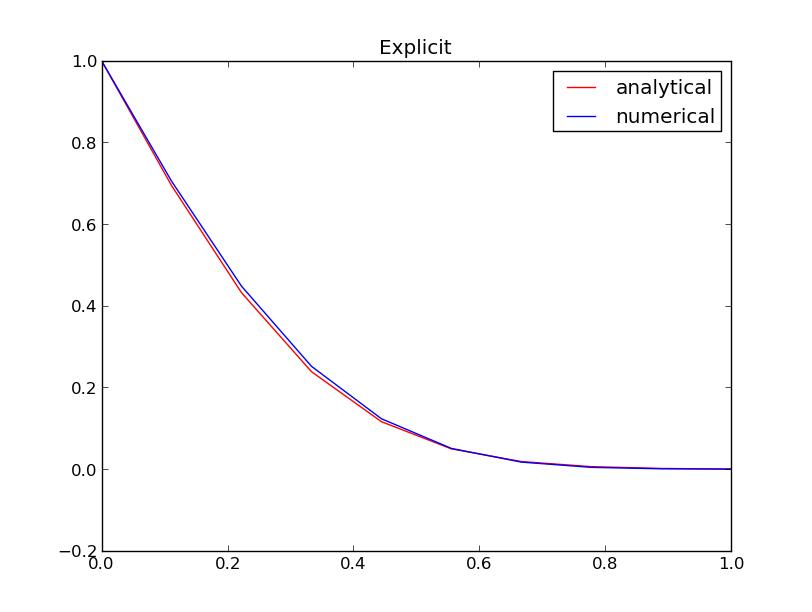
\includegraphics[scale=0.2]{stable_explicit.jpg}}
 \subfigure[dt = 0.005, Elapsed seconds = 2.44e-05]{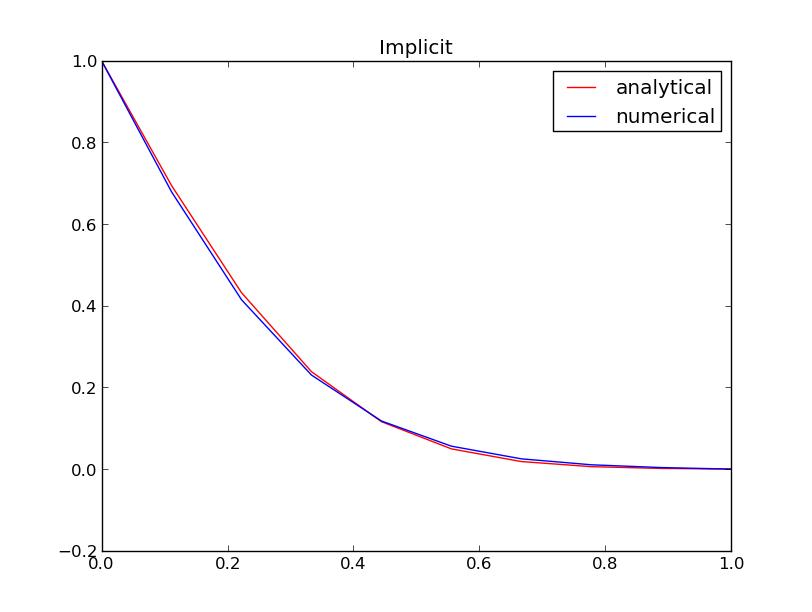
\includegraphics[scale=0.2]{stable_implicit.jpg}}
 \subfigure[dt = 0.005, Elapsed seconds = 3.0772e-05]{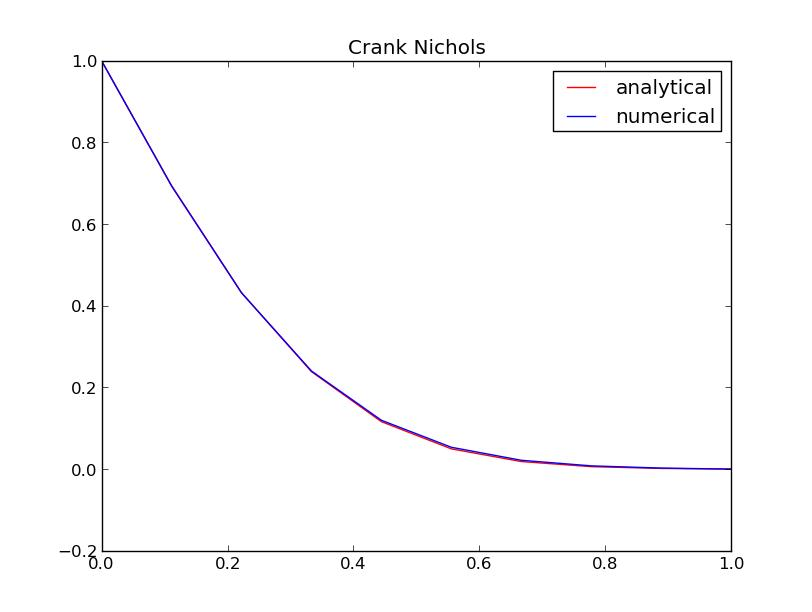
\includegraphics[scale=0.2]{stable_crank.jpg}}
 \end{center}
 \caption{\textit{plot of the different numerical solvers vs closed form solution}}
 \label{fig:edge}
\end{figure}

We can see from the plots of the different numerical solvers that the Crank Nichols scheme is the best in regards of error. But most 
interesting is that the Crank Nichols solver is as fast as the others, even faster than the explicit solver. This might not always
be the case, but at least it shows that it is not perceptibly slower, and therefore by far the best scheme.


\subsection*{1+1 Dimensional Diffusion equation, Markov Chains}

For the Markov Chains in 1+1 dimensions i found it quite hard to get the same plot for both fixed step length and gaussian step length.
The two simulations are fairly similar, but the gaussian seems to somehow develop slower in time. My guess is that this is due to
it somehow moving less particles out of the first step length per time step, and therefore adding less particles per time step.


\subsection*{}
\begin{figure}[H]
 \begin{center}
 \subfigure[$l_0 = 0.1$, Elapsed seconds = 0.65946]{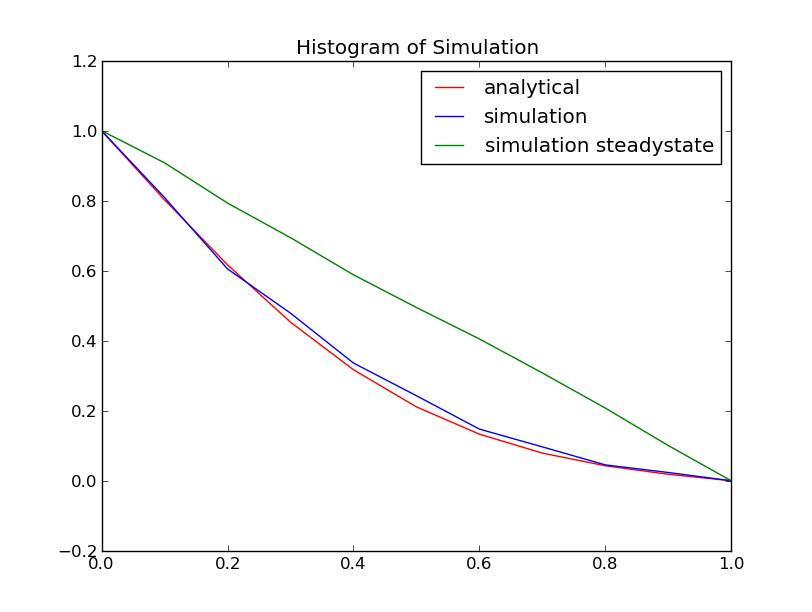
\includegraphics[scale=0.2]{1d_fixed.jpg}}
 \subfigure[$l_0 = 0.1$, Elapsed seconds = 1.21014]{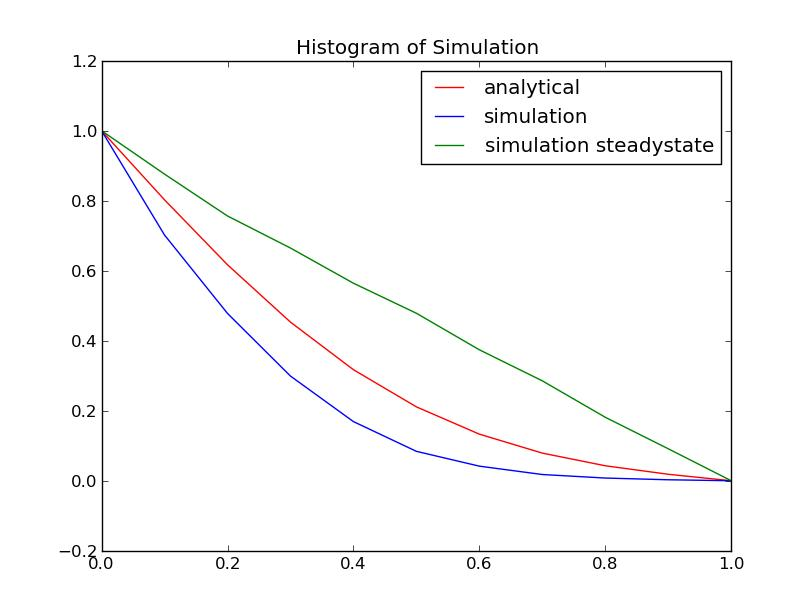
\includegraphics[scale=0.2]{1d_gauss.jpg}}
 \end{center}
 \caption{\textit{plot of the different 1+1 dimensional Markov Chain simulators vs closed form solution, $l_0 = 0.1$, $dt = {l_0}^2 /2$}}
 \label{fig:edge}
\end{figure}

We immediately find out that the simulations are way more resource demanding than the explicit and implicit solvers. They seem to
use at least a factor $10^5$ more time. And that is only for running the simulation once. What we wish to do is run the simulation several
times and take the mean value to get a good estimate.


\subsection*{2+1 Dimensional Diffusion equation}

Lets first take a look at the closed form solution to the Laplace equation. 

\subsection*{}
\begin{figure}[H]
 \begin{center}
 \subfigure[ ]{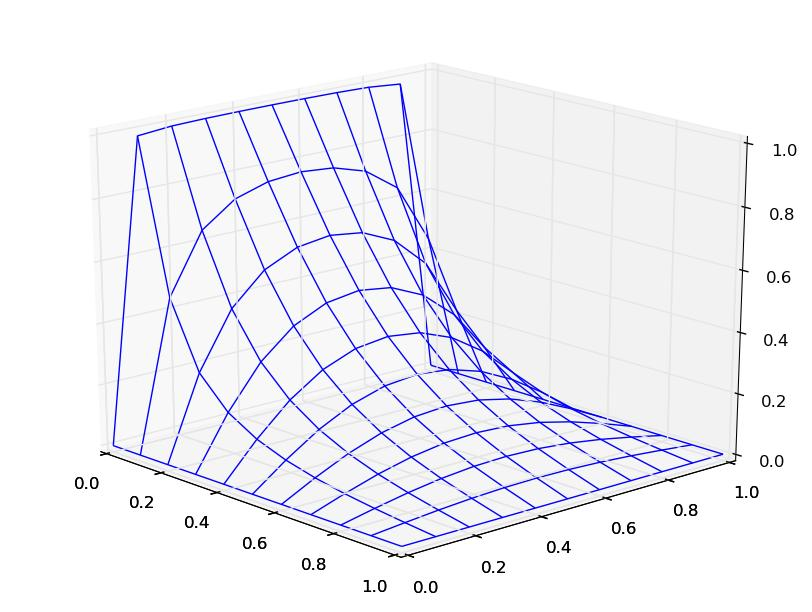
\includegraphics[scale=0.23]{2d_closedform.jpg}}
 \subfigure[ ]{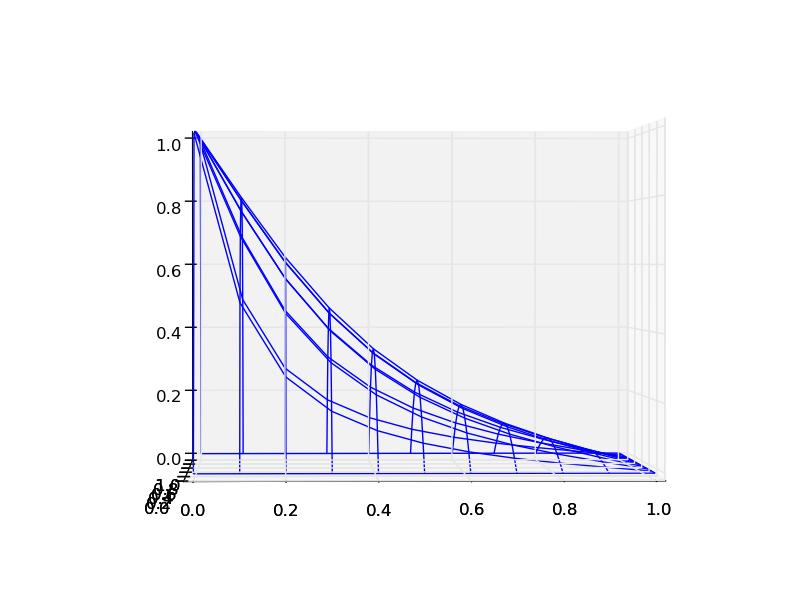
\includegraphics[scale=0.23]{2d_closedform2.jpg}}
 \end{center}
 \caption{\textit{plot of the closed form solution to the Laplace equation}}
 \label{fig:edge}
\end{figure}

We will use this plot as a reference to see if the other solutions make sense.

For the explicit scheme we need to be careful with stability. In 1+1 dimensions we need $\alpha \geq \frac{1}{2}$ in two dimensions,
as it turns out, we need $\alpha \geq \frac{1}{4}$. Where $\alpha = \frac{\Delta t}{\Delta x^2}$
\subsection*{}
\begin{figure}[H]
 \begin{center}
 \subfigure[ ]{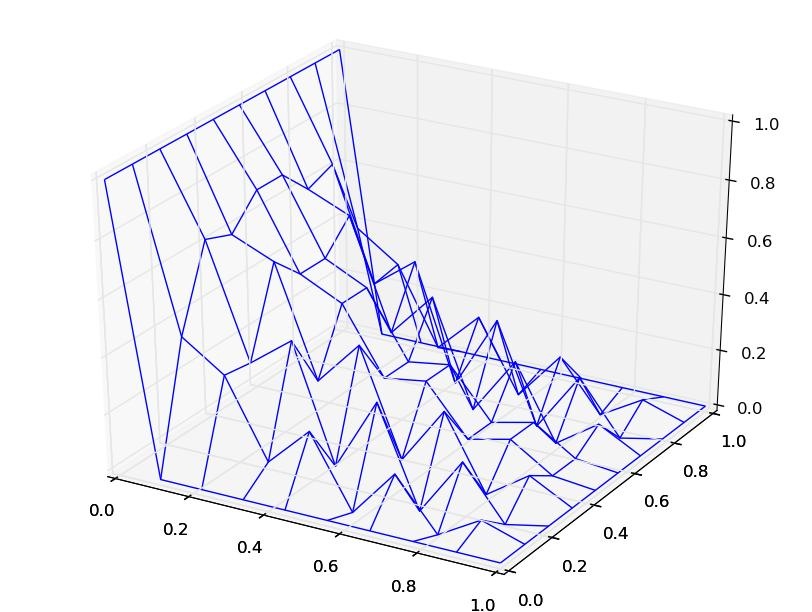
\includegraphics[scale=0.2]{2d_Explicit_unstable.jpg}}
 \end{center}
 \caption{\textit{plot of explicit solver with unstable $\alpha$}}
 \label{fig:edge}
\end{figure}


\subsection*{}
\begin{figure}[H]
 \begin{center}
 \subfigure[ ]{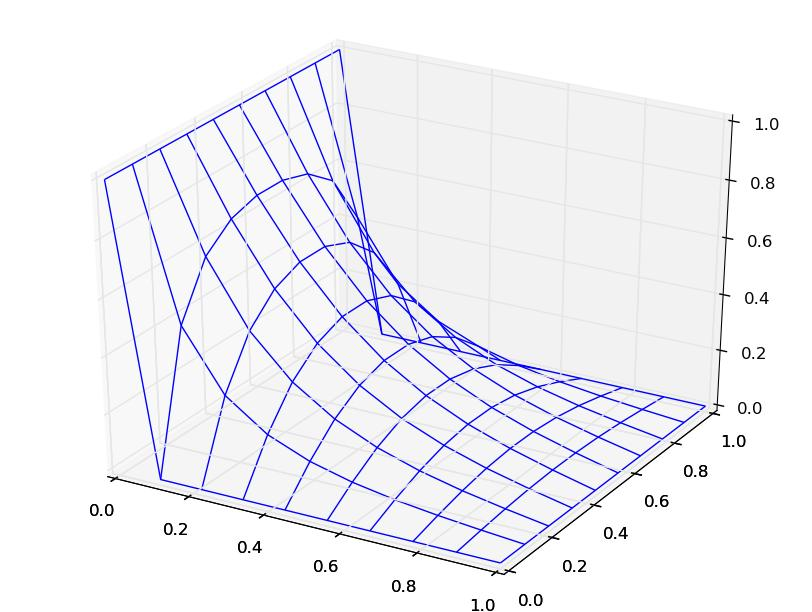
\includegraphics[scale=0.23]{2d_Explicit_diffsolv1.jpg}}
 \subfigure[ ]{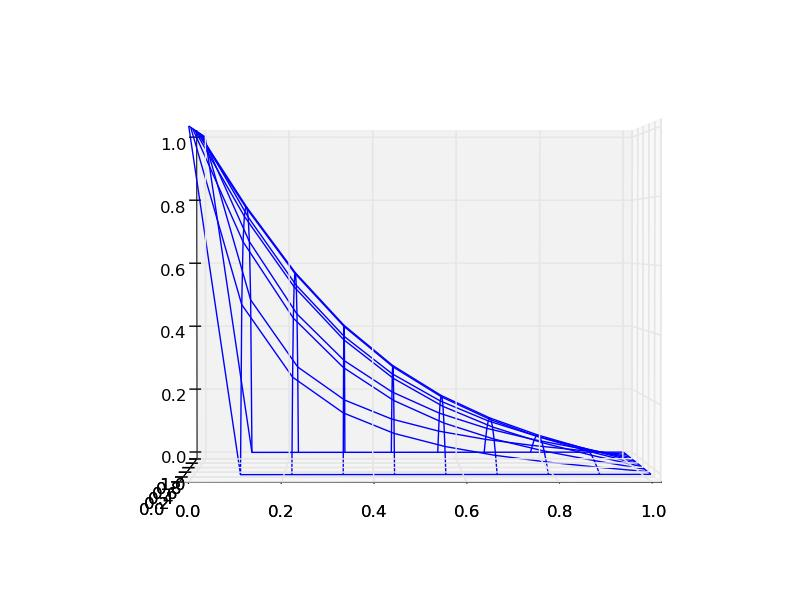
\includegraphics[scale=0.23]{2d_Explicit_diffsolv2.jpg}}
 \end{center}
 \caption{\textit{plot of explicit solver after reaching a steady state,  Elapsed seconds = 0.0106407}}
 \label{fig:edge}
\end{figure}

But with a stable $\alpha$ we can see that the explicit solver is doing exactly what it should.

The Implicit scheme also seems to do what we by now expect it to do.

\subsection*{}
\begin{figure}[H]
 \begin{center}
 \subfigure[ ]{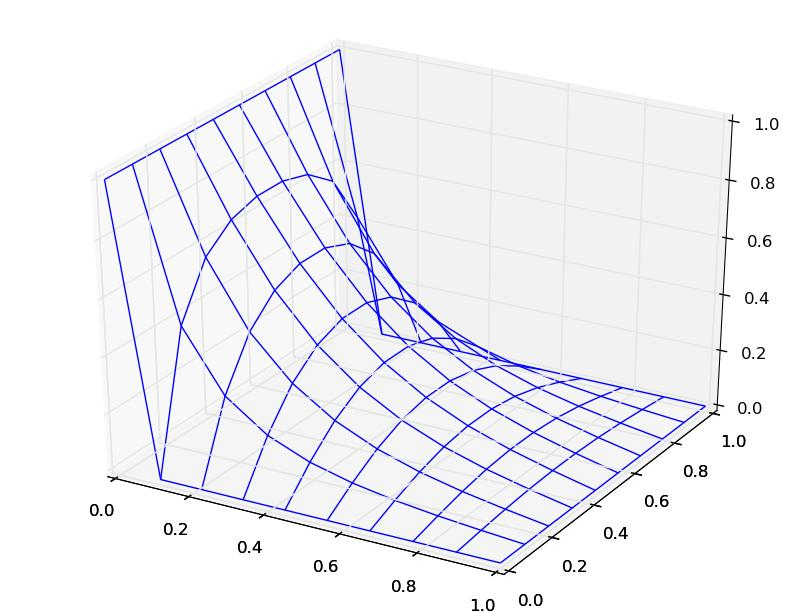
\includegraphics[scale=0.23]{2d_Implicit_diffsolv1.jpg}}
 \subfigure[ ]{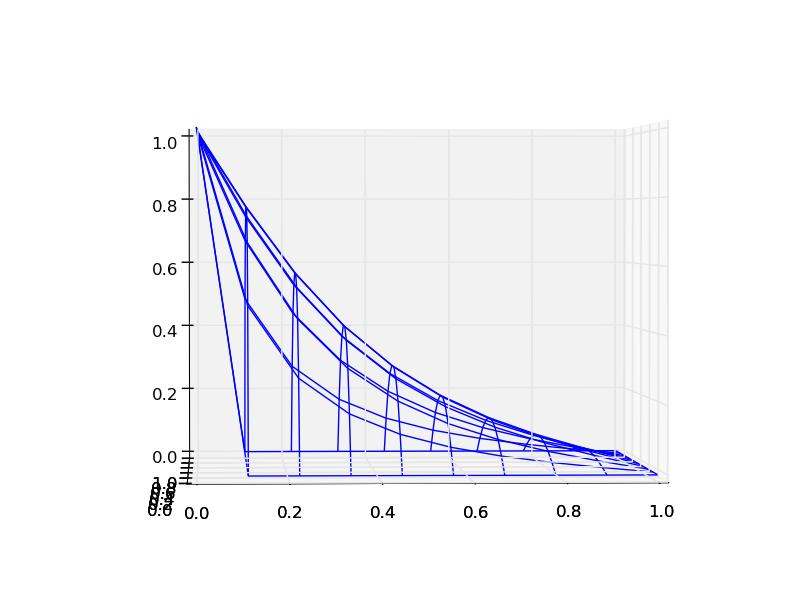
\includegraphics[scale=0.23]{2d_Implicit_diffsolv2.jpg}}
 \end{center}
 \caption{\textit{plot of Implicit solver after reaching a steady state,  Elapsed seconds =  0.0109125}}
 \label{fig:edge}
\end{figure}

The implicit scheme in contrast to the explicit seems to be allot more stable. The one big drawback to the Explicit scheme is the
stability issue, which is fine if we can control it. But in the case we are computing large data sets we will be bound by the stability.
In the implicit scheme we don't seem to have this problem. And all this goodness in the same time as the explicit scheme. 


\subsection*{2+1 Dimensional Diffusion equation,  Markov Chains}

And finally for the results of the Markov chain simulations.  

\subsection*{}
\begin{figure}[H]
 \begin{center}
 \subfigure[ ]{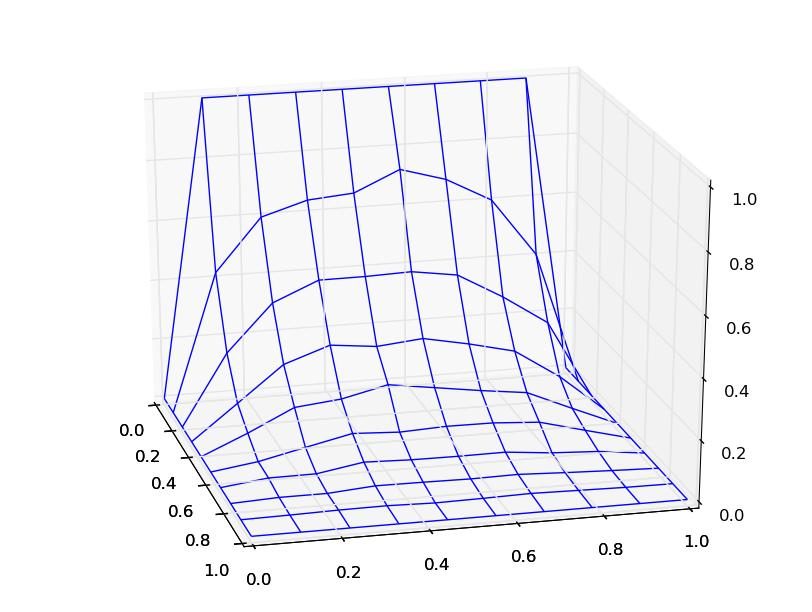
\includegraphics[scale=0.23]{2d_MC_10000_fixed.jpg}}
 \subfigure[ ]{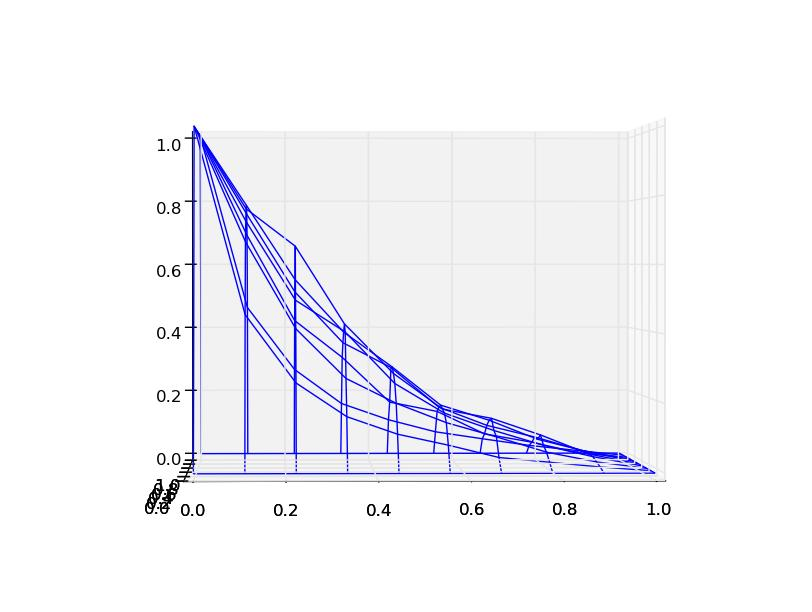
\includegraphics[scale=0.23]{2d_MC_10000_fixed2.jpg}}
 \end{center}
 \caption{\textit{plot of 2+1 dimensional Markov chain simulation, fixed step length $l_0 = 0.1$, Elapsed seconds =  0.60721}}
 \label{fig:edge}
\end{figure}

\subsection*{}
\begin{figure}[H]
 \begin{center}
 \subfigure[ ]{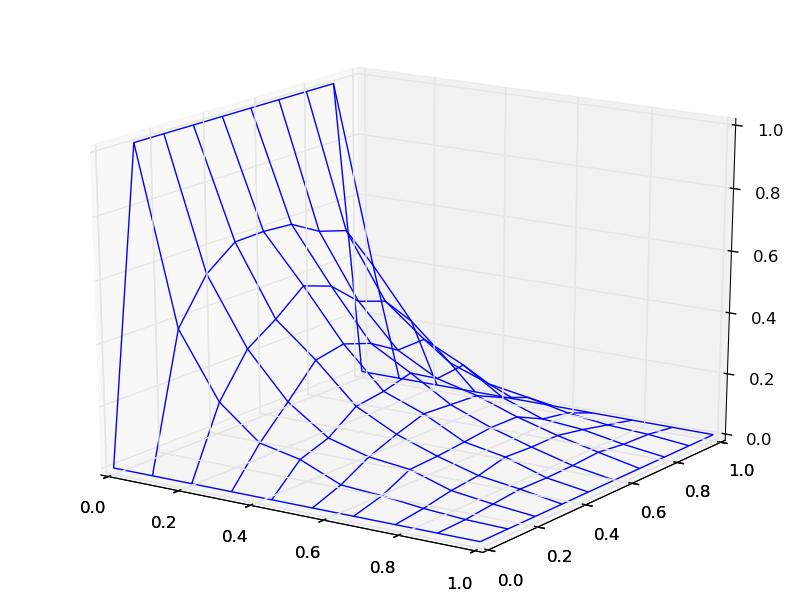
\includegraphics[scale=0.23]{2d_MC_10000_gauss.jpg}}
 \subfigure[ ]{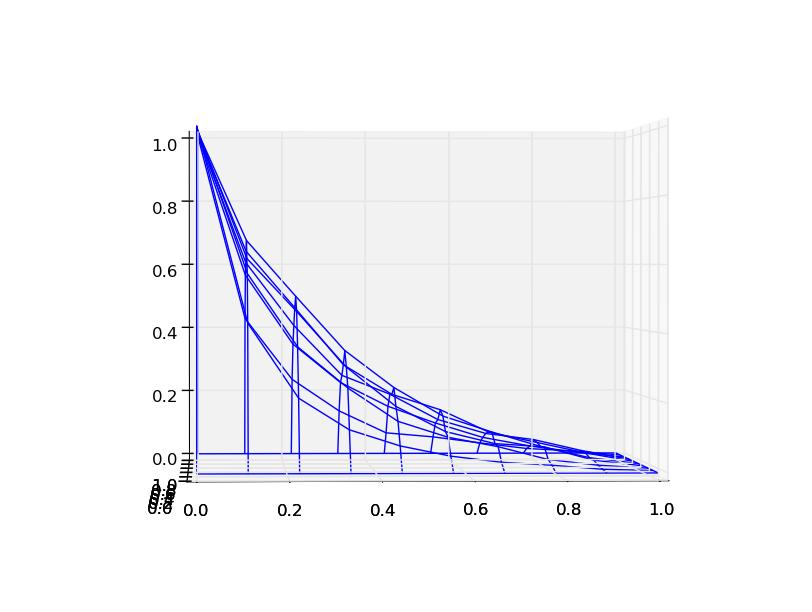
\includegraphics[scale=0.23]{2d_MC_10000_gauss2.jpg}}
 \end{center}
 \caption{\textit{plot of 2+1 dimensional Markov chain simulation, random normal distributed step length $l_0 = 0.1$, Elapsed seconds =  1.15229}}
 \label{fig:edge}
\end{figure}

In both the random and fixed step lengths we see that they are for the most part doing what they should. In these plots i ran the 
simulation only once. As a result of that we can see some discrepancies in the plot, that is the lines are not totally smooth. 
For this to be a good Monte Carlo simulation with perfect plots we would have to run the simulations several times and take the mean values. Or run the simulation
with allot more particles. I chose to use these plots because they show that the system works and is much closer to the numerical solvers
in regards of resources. The times are stated under the plots.

To show that the system can give smooth lines will add a last plot with 10 times more particles

\subsection*{}
\begin{figure}[H]
 \begin{center}
 \subfigure[ ]{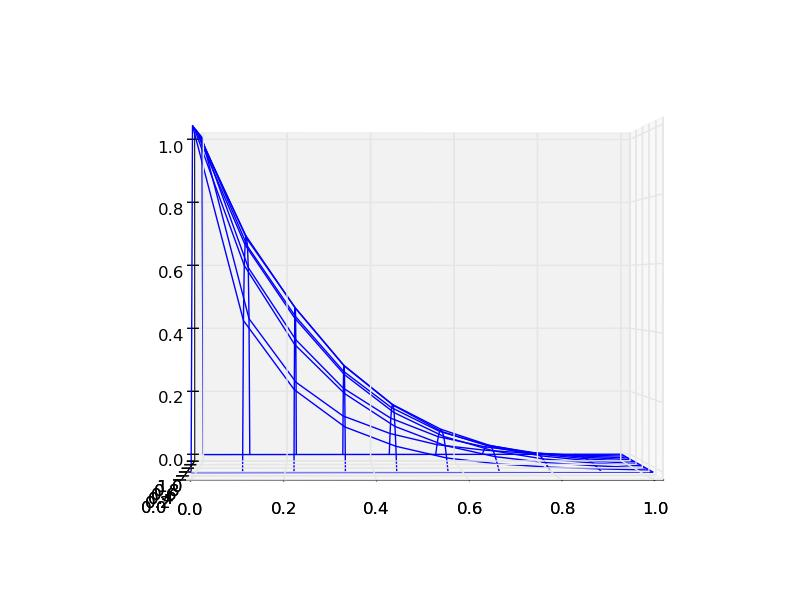
\includegraphics[scale=0.3]{2d_MC_100000_gauss_2.jpg}}
 \end{center}
 \caption{\textit{plot of 2+1 dimensional Markov chain simulation, random normal distributed step length $l_0 = 0.1$, $N=10^5$}}
 \label{fig:edge}
\end{figure}


\section*{Conclusion}

In one spatial dimension we have seen that it indeed is possible to simulate diffusion and produce a result that is similar to
a closed form solution. I think it is safe to say that this method is not the most effective for most purposes since it was $10^5$ times slower at best.
In our case we were able to solve the equation numerically with an implicit and explicit scheme, which both where much faster.

I found it hard to differentiate the random and fixed step length in 2+1 dimension Markov chains. They both behave in fairly the same way.
But the random step length one used almost double the time of the fixed step length one. So that gives one point in favour of the
fixed step length. One can argue though that the normal distributed step length is more physically correct.

We also solved the 2+1 dimensional equation with an explicit and implicit scheme. With both these we saw that they were still faster
than the Markov chains. They used about the same time, and i would therefore recommend the implicit scheme. Based on the plots they
seem to have similar errors, but the implicit has one huge advantage in stability. The gap between the PDE solvers and the Markov chains
has been a little bridged, but the Markov chains are still slow in comparison. Maybe this will get even better in 3+1 dimensions?


%\newpage


%\section*{Attachments}
%\textbf{Attachment 1: C++ main program}\newline
%\lstinputlisting[language=C++]{main.cpp}
%\newpage
\end{document}
